\begin{frame}
    \frametitle{Analyzing Unknown Formats}

    \begin{itemize}
        \item Threat actors often use customized binary formats for encoding.
        \item Malware configuration parsing\footnote{\url{https://github.com/TeamT5/MalCfgParser}}.
        \item Beacons of remote access tools, such as Cobalt Strike.
    \end{itemize}
    \centering
    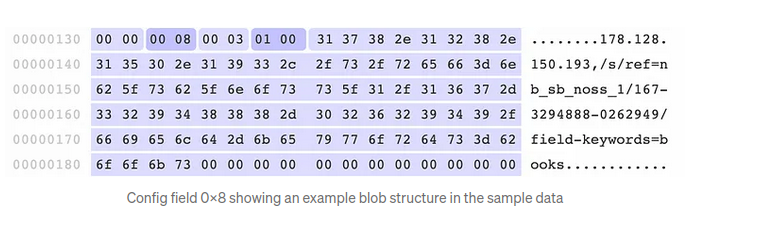
\includegraphics[scale=0.5]{img/cobalt.png}
    Image source:\footnote{\url{https://sixdub.medium.com/using-kaitai-to-parse-cobalt-strike-beacon-configs-f5f0552d5a6e}}.
\end{frame}


\begin{frame}[fragile]
\frametitle{Setting up Kaitai Struct}

\begin{itemize}
    \item The latest release (as of 2022) is available on GitHub:
          \url{https://github.com/kaitai-io/kaitai_struct}.
    \item To build Kaitai Struct from sources:
          \begin{itemize}
              \item Ensure you have \textbf{Scala SBT (sbt)} installed.
              \item Clone the repository and run the build commands.
          \end{itemize}
    \item Command sequence for building Kaitai Struct.
\end{itemize}


\lstdefinelanguage{bash}{
    keywords={git, sbt, clone, push, pull, add, commit, checkout, branch},
    keywordstyle=\color{blue}\bfseries,
    ndkeywords={https, recursive, universal, packageBin, compile},
    ndkeywordstyle=\color{teal}\bfseries,
    identifierstyle=\color{black},
    sensitive=false,
    comment=[l]{\#},
    commentstyle=\color{gray}\itshape,
    stringstyle=\color{orange},
    showstringspaces=false,
    basicstyle=\ttfamily\small,
    morestring=[b]"
}

\lstset{
    language=bash,
    breaklines=true,        % Enable line breaking
    breakatwhitespace=true, % Break lines at spaces
    prebreak=\textbackslash, % Add '\' at line breaks
    postbreak=\space        % Add a space after line breaks
}

\begin{lstlisting}[language=bash]
git clone --recursive https://github.com/kaitai-io/kaitai_struct.git
sbt compile
sbt compilerJVM/universal:packageBin
unzip unpack the zip file in kaitai_struct/compiler/jvm/target/universal/kaitai-struct-compiler-0.11-SNAPSHOT.zip

kaitai-struct-compiler -h

\end{lstlisting}


\end{frame}

\lstdefinelanguage{bash}{
    keywords={python3,source,pip3},
    keywordstyle=\color{blue}\bfseries,
    ndkeywords={https, recursive, universal, packageBin, compile},
    ndkeywordstyle=\color{teal}\bfseries,
    identifierstyle=\color{black},
    sensitive=false,
    comment=[l]{\#},
    commentstyle=\color{gray}\itshape,
    stringstyle=\color{orange},
    showstringspaces=false,
    basicstyle=\ttfamily\small,
    morestring=[b]"
}


\begin{frame}[fragile]
    \frametitle{Setting up Kaitai Struct Python Environment}

    To set up the Python environment for Kaitai Struct, follow these steps:



    \begin{lstlisting}[language=bash,frame=single]
python3 -m venv venv
source venv/bin/activate
pip3 install kaitaistruct
python3 parse.py
    \end{lstlisting}

    \textbf{Important:} Ensure you stay within the virtual environment. Exiting the virtual environment may prevent your script from running as expected.
\end{frame}

% Define YAML language style with proper coloring for keywords
\lstdefinelanguage{yaml}{
    keywords={true, false, null, yes, no},
    keywordstyle=\color{blue}\bfseries,
    basicstyle=\ttfamily\footnotesize,
    comment=[l]{\#},
    commentstyle=\color{green!50!black},
    stringstyle=\color{orange},
    morekeywords={meta, id, title, endian, seq, type, size}, % Add YAML keys for highlighting
    moredelim=**[il][\color{black}]{---},   % Highlight YAML start
    moredelim=**[il][\color{black}]{...},   % Highlight YAML end
    showstringspaces=false,
    breaklines=true,
    frame=single,
}

\definecolor{offsetcolor}{rgb}{1.0, 0.6, 0.6}  % Light red
\definecolor{headercolor}{rgb}{0.7, 0.85, 1.0} % Light blue
\definecolor{bodycolor}{rgb}{1.0, 0.85, 0.4}   % Light gold

\begin{frame}[fragile]{Custom Format used in Kaitai Struct Example}
The following is an example of a `.ksy` file for Kaitai Struct:

\begin{table}
\centering
\renewcommand{\arraystretch}{1.5} % Increase row height
\begin{tabular}{|c|c|c|}
\hline
\textbf{Offset (Bytes)} & \textbf{Field Name} & \textbf{Description} \\ \hline
0x00--0x03             & \cellcolor{headercolor} Header              & 4-byte unsigned integer (u4) \\ \hline
0x04--0x0A             & \cellcolor{bodycolor} Body                & 8 bytes of data              \\ \hline
\end{tabular}
\caption{Structure of the Example Data Format}
\end{table}

%02d2 4996 6261 6463 6665 6867
\begin{table}
\scalebox{0.95}{
\centering
\begin{tabular}{|l|l|l|l|l|l|l|l|l|l|l|l|l|}
\hline
Offset & 00 & 01 & 02 & 03 & 04 & 04 & 05 & 06 & 07 & 08 & 09 & A\\
\hline
Content & \cellcolor{headercolor} 02 & \cellcolor{headercolor} d2 & \cellcolor{headercolor} 49 & \cellcolor{headercolor}96 & \cellcolor{bodycolor} 62 & \cellcolor{bodycolor} 61 & \cellcolor{bodycolor}64 & \cellcolor{bodycolor}63 & \cellcolor{bodycolor}66 & \cellcolor{bodycolor}65 & \cellcolor{bodycolor}68 & \cellcolor{bodycolor}67\\
\hline
\end{tabular}
}
\caption{Visualization of the Example File}
\end{table}

\end{frame}

\begin{frame}[fragile]
\frametitle{Description of custom binary format in YAML}

Create an example.ksy file

\begin{lstlisting}[language=yaml]
meta:
  id: example
  title: Example Binary Format
  endian: le
seq:
  - id: header
    type: u4
  - id: body
    size: 8
\end{lstlisting}

Transform it into python code

\begin{lstlisting}[language=bash,frame=single]
kaitai-struct-compiler -t python example.ksy
\end{lstlisting}
\end{frame}

\begin{frame}[fragile]
\frametitle{Generated Python File}

\lstset{
    language=Python,
    basicstyle=\ttfamily\footnotesize,
    keywordstyle=\color{blue}\bfseries,
    commentstyle=\color{green!50!black},
    stringstyle=\color{orange},
    showstringspaces=false,
    breaklines=true,
    frame=single,
}

\begin{lstlisting}
# This is a generated file! Please edit source .ksy file and use kaitai-struct-compiler to rebuild

import kaitaistruct
from kaitaistruct import KaitaiStruct, KaitaiStream, BytesIO

class Example(KaitaiStruct):
    def __init__(self, _io, _parent=None, _root=None):
        self._io = _io
        self._parent = _parent
        self._root = _root if _root else self
        self._read()

    def _read(self):
        self.header = self._io.read_u4le()
        self.body = self._io.read_bytes(8)

\end{lstlisting}
\end{frame}


\begin{frame}[fragile]
\frametitle{Using your generated python class}

\lstset{
    language=Python,
    basicstyle=\ttfamily\footnotesize,
    keywordstyle=\color{blue}\bfseries,
    commentstyle=\color{green!50!black},
    stringstyle=\color{orange},
    showstringspaces=false,
    breaklines=true,
    frame=single,
}
\begin{lstlisting}
from example import Example

# Open the binary file
with open("data.bin", "rb") as f:
    data = Example.from_io(f)

# Access parsed fields
print(f"Header: {data.header}")
print(f"Body: {data.body}")
\end{lstlisting}
\end{frame}

\begin{frame}
\frametitle{Kaitai Struct Formats - Overview}

\begin{itemize}
    \item The Kaitai Struct community actively \textbf{publishes} formats that can be parsed using Kaitai Struct.
    \item Explore available formats:
          \begin{itemize}
              \item Community repository: \url{https://github.com/kaitai-io/kaitai_struct_formats/}
              \item Example: Parsing ELF files:
                    \url{https://github.com/kaitai-io/kaitai_struct_formats/blob/master/executable/elf.ksy}
          \end{itemize}
    \item Formats cover a wide range of applications, including:
          \begin{itemize}
              \item Databases
              \item Windows-related formats
              \item Serialization
              \item Security
              \item Networking
              \item Media
              \item MacOS
              \item Filesystems
          \end{itemize}
\end{itemize}

\end{frame}

\begin{frame}
\frametitle{Kaitai Struct Formats - Categories (1/2)}

\begin{itemize}
    \item \textbf{Databases}:
          \begin{itemize}
              \item SQLite3
          \end{itemize}
    \item \textbf{Windows}:
          \begin{itemize}
              \item LNK files
              \item Minidump
              \item Shell items
              \item System time
              \item Registry
          \end{itemize}
    \item \textbf{Serialization}:
          \begin{itemize}
              \item BSON
              \item Chrome
              \item Google Protobuf
              \item Microsoft CFB
              \item MGSPack
              \item PHP serialized
              \item Python CPickle
              \item Ruby Marshal
          \end{itemize}
\end{itemize}
\end{frame}

\begin{frame}
\frametitle{Kaitai Struct Formats - Categories (2/2)}

\begin{itemize}
    \item \textbf{Security}:
          \begin{itemize}
              \item EFI variable signature
              \item SSH public key
          \end{itemize}
    \item \textbf{Networking}:
          \begin{itemize}
              \item Bitcoin transaction key
              \item WebSocket
          \end{itemize}
    \item \textbf{Media}:
          \begin{itemize}
              \item Android OpenGL shaders cache
              \item WAV
          \end{itemize}
    \item \textbf{MacOS}:
          \begin{itemize}
              \item DS\_Store
              \item Mac OS resource
          \end{itemize}
    \item \textbf{Filesystems}:
          \begin{itemize}
              \item LUKS
              \item VDI
          \end{itemize}
\end{itemize}

\end{frame}

